\section{Interprocedural Profiling}

\ifdefined\noauthorea
\begin{figure}[hb]
\begin{center}
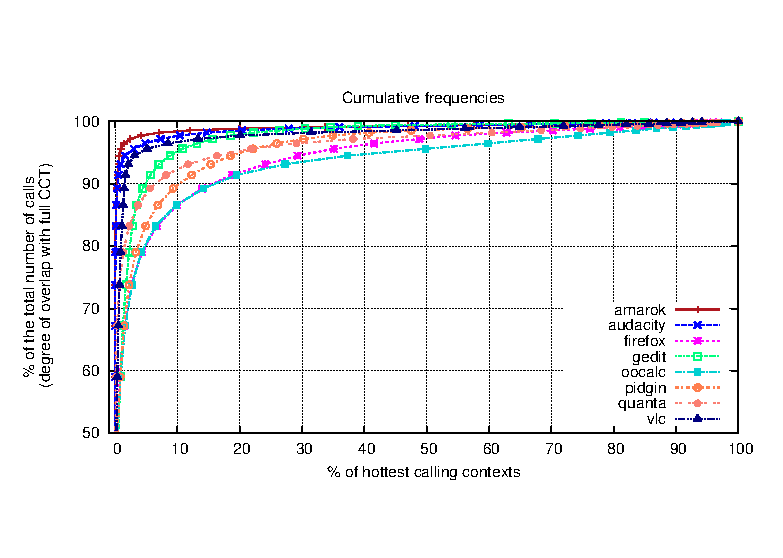
\includegraphics[width=0.95\columnwidth]{figures/hcct-skewness/hcct-skewness.eps}
\caption{\protect\label{fig:hcct-skewness} Skewness of calling contexts distribution on a representative subset of applications. For instance, in {\tt oocalc}, 10\% of the hottest calling contexts account for more than 86\% of all routine calls.
}
\end{center}
\end{figure}
\fi

Lorem ipsum...
%~\cite{}

%Context-sensitive profiling provides 
%These algorithms allow us to distinguish between hot and cold context on-the-fly, and we show both theoretically and experimentally that for collected metrics the HCCT achieves a similar precision as the CCT in a space that is several orders of magnitude smaller. We show on prominent benchmarks that our implementation, shipping as a plugin for the \gcc\ compiler, incurs a slowdown competitive with the \gprof\ profiler while collecting much finer-grained profiles.

\subsection{Approach}

\subsection{Algorithms}

\subsection{Implementation}

\subsection{Comparison with Related Work}

\subsection{Discussion}
